% Per-method interconnect regions: region cutting, per-method checks,
% cross-method check and the unclaimed remainder.
\documentclass[border=4pt]{standalone}
\usepackage{tikz}
\usetikzlibrary{arrows.meta, positioning, calc}
\usepackage[T1]{fontenc}
\usepackage{lmodern}

% IHP palette, matching the other figures in this directory.
\definecolor{IHPfg}{RGB}{0,80,139}
\definecolor{IHPaccent}{RGB}{109,112,114}
\definecolor{cCuPillar}{RGB}{184,115,51}
\definecolor{cChiplet}{RGB}{55,145,195}
\definecolor{cCross}{RGB}{140,55,140}

\begin{document}
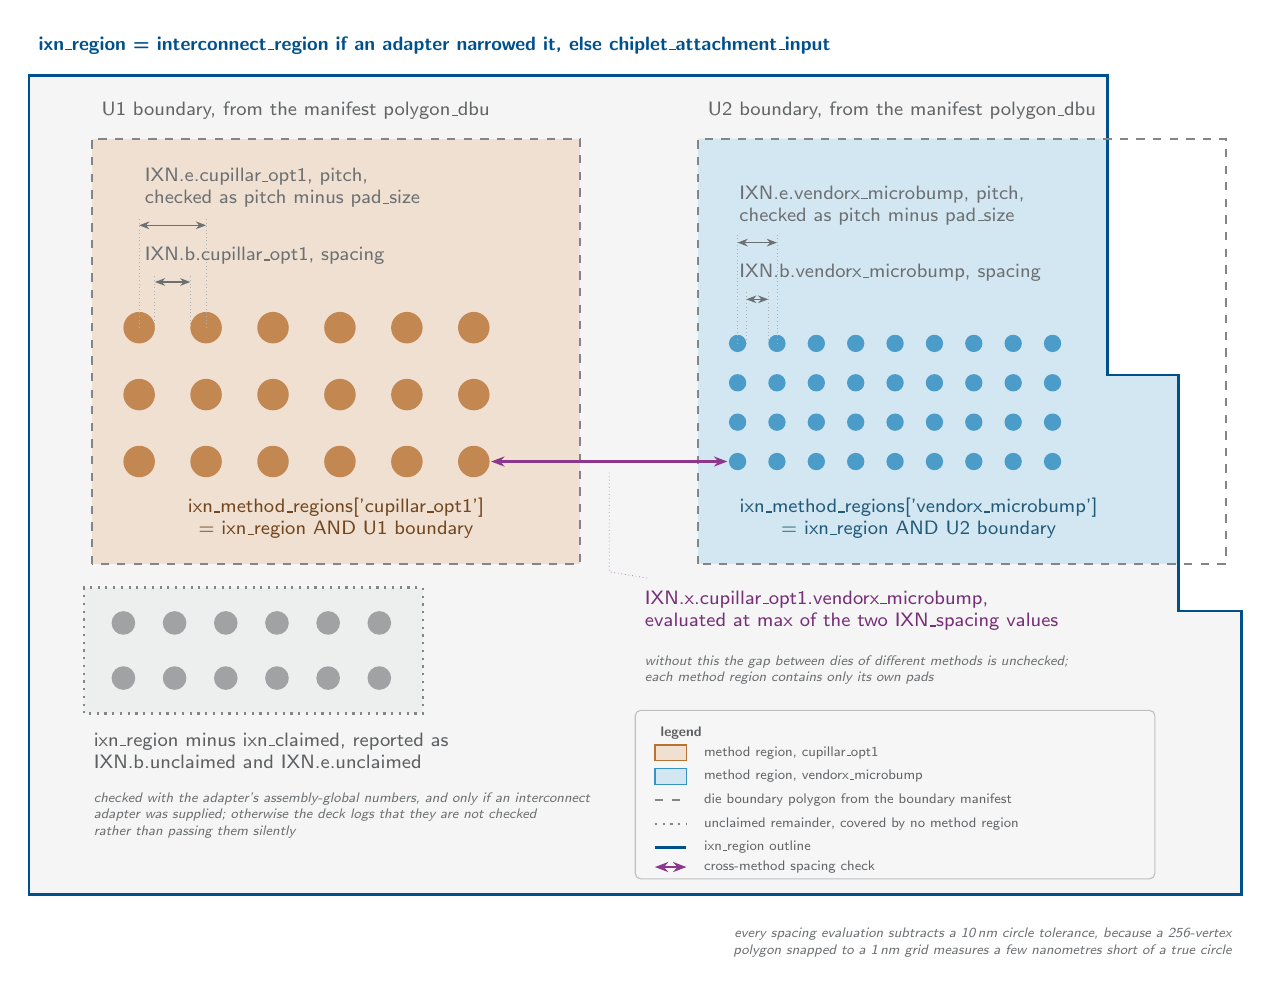
\begin{tikzpicture}[
    x=1cm, y=1cm,
    >=Stealth,
    adkreglbl/.style={font=\sffamily\scriptsize, text=#1, align=center},
    adkreglbl/.default=IHPaccent,
    adkdielbl/.style={font=\sffamily\scriptsize, text=IHPaccent!90!black,
                      anchor=south west, align=left},
    adkdim/.style={{Stealth[length=1.3mm]}-{Stealth[length=1.3mm]},
                   line width=0.5pt, color=IHPaccent},
    adkext/.style={line width=0.3pt, color=IHPaccent!55, densely dotted},
    adkchk/.style={font=\sffamily\scriptsize, text=#1,
                   anchor=south west, align=left},
    adkchk/.default=IHPaccent,
    adkcross/.style={{Stealth[length=1.7mm]}-{Stealth[length=1.7mm]},
                     line width=0.8pt, color=cCross},
    adkcallout/.style={font=\sffamily\tiny\itshape, text=IHPaccent,
                       anchor=north west, align=left},
    adklead/.style={line width=0.3pt, color=cCross!60, densely dotted},
    adklegtxt/.style={font=\sffamily\tiny, text=IHPaccent!90!black, anchor=west}
]

% ======================================================================
% Outer region: ixn_region, with an irregular right edge
% ======================================================================
\def\adkouter{(0,0) -- (15.4,0) -- (15.4,3.6) -- (14.6,3.6) --
              (14.6,6.6) -- (13.7,6.6) -- (13.7,10.4) -- (0,10.4) -- cycle}

\fill[IHPaccent!7] \adkouter;

% ---- method region A: ixn_region AND U1 boundary (fully inside) ----
\fill[cCuPillar!22] (0.8,4.2) rectangle (7.0,9.6);

% ---- method region B: ixn_region AND U2 boundary (clipped on the right) ----
\fill[cChiplet!22] (8.5,4.2) -- (14.6,4.2) -- (14.6,6.6) -- (13.7,6.6) --
                   (13.7,9.6) -- (8.5,9.6) -- cycle;

% ---- outer outline on top of the tints ----
\draw[IHPfg, line width=0.9pt] \adkouter;
\node[font=\sffamily\scriptsize\bfseries, text=IHPfg, anchor=south west]
    at (0,10.55)
    {ixn\_region = interconnect\_region if an adapter narrowed it, else chiplet\_attachment\_input};

% ---- die boundaries from the manifest ----
\draw[IHPaccent!85, dashed, line width=0.7pt] (0.8,4.2) rectangle (7.0,9.6);
\draw[IHPaccent!85, dashed, line width=0.7pt] (8.5,4.2) rectangle (15.2,9.6);

\node[adkdielbl] at (0.8,9.72) {U1 boundary, from the manifest polygon\_dbu};
\node[adkdielbl] at (8.5,9.72) {U2 boundary, from the manifest polygon\_dbu};

% ======================================================================
% Attachment pads
% ======================================================================
% coarse and large, method A
\foreach \px in {1.4,2.25,3.1,3.95,4.8,5.65}
  \foreach \py in {5.5,6.35,7.2}
    \fill[cCuPillar!85] (\px,\py) circle (0.20);

% fine and small, method B
\foreach \px in {9.0,9.5,...,13.0}
  \foreach \py in {5.5,6.0,6.5,7.0}
    \fill[cChiplet!90] (\px,\py) circle (0.11);

% ======================================================================
% Method region labels
% ======================================================================
\node[adkreglbl=cCuPillar!62!black] at (3.9,4.78)
    {ixn\_method\_regions['cupillar\_opt1']\\= ixn\_region AND U1 boundary};
\node[adkreglbl=cChiplet!62!black] at (11.3,4.78)
    {ixn\_method\_regions['vendorx\_microbump']\\= ixn\_region AND U2 boundary};

% ======================================================================
% Per-method checks, region A
% ======================================================================
% spacing, edge to edge
\draw[adkext] (1.60,7.20) -- (1.60,7.88);
\draw[adkext] (2.05,7.20) -- (2.05,7.88);
\draw[adkdim] (1.60,7.78) -- (2.05,7.78);
\node[adkchk=IHPaccent] at (1.35,7.88) {IXN.b.cupillar\_opt1, spacing};

% pitch, centre to centre
\draw[adkext] (1.40,7.20) -- (1.40,8.60);
\draw[adkext] (2.25,7.20) -- (2.25,8.60);
\draw[adkdim] (1.40,8.50) -- (2.25,8.50);
\node[adkchk=IHPaccent] at (1.35,8.60)
    {IXN.e.cupillar\_opt1, pitch,\\checked as pitch minus pad\_size};

% ======================================================================
% Per-method checks, region B
% ======================================================================
\draw[adkext] (9.11,7.00) -- (9.11,7.66);
\draw[adkext] (9.39,7.00) -- (9.39,7.66);
\draw[adkdim] (9.11,7.56) -- (9.39,7.56);
\node[adkchk=IHPaccent] at (8.90,7.66) {IXN.b.vendorx\_microbump, spacing};

\draw[adkext] (9.00,7.00) -- (9.00,8.38);
\draw[adkext] (9.50,7.00) -- (9.50,8.38);
\draw[adkdim] (9.00,8.28) -- (9.50,8.28);
\node[adkchk=IHPaccent] at (8.90,8.38)
    {IXN.e.vendorx\_microbump, pitch,\\checked as pitch minus pad\_size};

% ======================================================================
% Cross-method check across the gap
% ======================================================================
\draw[adkcross] (5.87,5.5) -- (8.87,5.5);
\draw[adklead] (7.37,5.36) -- (7.37,4.10) -- (7.85,4.02);

\node[font=\sffamily\scriptsize, text=cCross!85!black,
      anchor=north west, align=left] at (7.70,3.98)
    {IXN.x.cupillar\_opt1.vendorx\_microbump,\\evaluated at max of the two IXN\_spacing values};

\node[adkcallout] at (7.70,3.16)
    {without this the gap between dies of different methods is unchecked;\\
     each method region contains only its own pads};

% ======================================================================
% Unclaimed remainder
% ======================================================================
\fill[IHPaccent!12] (0.70,2.30) rectangle (5.00,3.90);
\draw[IHPaccent!85, dotted, line width=0.8pt] (0.70,2.30) rectangle (5.00,3.90);

\foreach \px in {1.20,1.85,2.50,3.15,3.80,4.45}
  \foreach \py in {2.75,3.45}
    \fill[IHPaccent!65] (\px,\py) circle (0.15);

\node[font=\sffamily\scriptsize, text=IHPaccent!85!black,
      anchor=north west, align=left] at (0.70,2.18)
    {ixn\_region minus ixn\_claimed, reported as\\IXN.b.unclaimed and IXN.e.unclaimed};

\node[adkcallout] at (0.70,1.42)
    {checked with the adapter's assembly-global numbers, and only if an interconnect\\
     adapter was supplied; otherwise the deck logs that they are not checked\\
     rather than passing them silently};

% ======================================================================
% Inset legend
% ======================================================================
\draw[IHPaccent!45, line width=0.4pt, rounded corners=2pt, fill=IHPaccent!6]
    (7.70,0.20) rectangle (14.30,2.34);
\node[font=\sffamily\tiny\bfseries, text=IHPaccent!85!black, anchor=north west]
    at (7.90,2.26) {legend};

\fill[cCuPillar!22] (7.95,1.70) rectangle (8.35,1.90);
\draw[cCuPillar, line width=0.5pt] (7.95,1.70) rectangle (8.35,1.90);
\node[adklegtxt] at (8.45,1.80) {method region, cupillar\_opt1};

\fill[cChiplet!22] (7.95,1.40) rectangle (8.35,1.60);
\draw[cChiplet, line width=0.5pt] (7.95,1.40) rectangle (8.35,1.60);
\node[adklegtxt] at (8.45,1.50) {method region, vendorx\_microbump};

\draw[IHPaccent!85, dashed, line width=0.7pt] (7.95,1.20) -- (8.35,1.20);
\node[adklegtxt] at (8.45,1.20) {die boundary polygon from the boundary manifest};

\draw[IHPaccent!85, dotted, line width=0.8pt] (7.95,0.90) -- (8.35,0.90);
\node[adklegtxt] at (8.45,0.90) {unclaimed remainder, covered by no method region};

\draw[IHPfg, line width=0.9pt] (7.95,0.60) -- (8.35,0.60);
\node[adklegtxt] at (8.45,0.60) {ixn\_region outline};

\draw[adkcross] (7.95,0.35) -- (8.35,0.35);
\node[adklegtxt] at (8.45,0.35) {cross-method spacing check};

% ======================================================================
% Tolerance note
% ======================================================================
\node[font=\sffamily\tiny\itshape, text=IHPaccent, anchor=north east,
      align=right] at (15.40,-0.30)
    {every spacing evaluation subtracts a 10\,nm circle tolerance, because a 256-vertex\\
     polygon snapped to a 1\,nm grid measures a few nanometres short of a true circle};

\end{tikzpicture}
\end{document}
